\subsection{Matter}

\begin{enumerate}
	\item Categorize the following changes as either chemical or physical: Freezing of juice in a bottle, Rusting of iron, Burning of wood, Drying of wet clothes
	
	\item Give three difference between the following: Compound and mixture, Suspension and solution
	
	\item The figure below shows the relationship among three states of matter. Name the processes involved in A, B, C, and D.
	\vspace*{-7mm}
	\begin{center}
		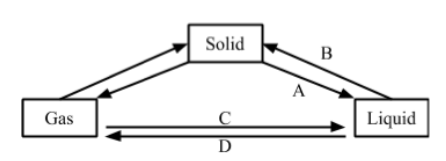
\includegraphics[width=0.6\textwidth]{./img/chem_I_matter_1.png}
	\end{center}
	
	\item Match each item in List A with the correct response in List B
	\begin{center}
		\begin{tabular}{|cp{8cm}|cp{3cm}|} \hline
			\multicolumn{2}{|c|}{List A} & \multicolumn{2}{|c|}{List B} \\ \hline
			I) & A process of separating a mixture of sodium chloride & A & Evaporation \\ 
			&  and ammonium chloride & B & Filtration \\
			II) & A method used to separate oil and water & C & Boiling \\
			III) & A method by which coloured substances are & D & Chrmoatography \\
			&  separated and identified & E & Distillation \\
			IV) & A method by which salt and water can be separated & F & Layer separation \\
			V) &  A method used to get the solvent from the solution & G & Decantation \\ 
			&  mixture & H & Sublimation \\ \hline
		\end{tabular}
	\end{center}
	
	\item Define matter
	
	\item Tell whether the following is a chemical change or physical change: Rotting of mango; Clouds changing into rain; Decaying of teeth
	
	\item State four difference between a chemical change and physical change
	
	\item The following figure shows the apparatus that can be used to separate three liquids: cooking oil, kerosene and water with density 0.92 g/cm$^3$, 0.65 g/cm$^3$, and 1.00 g/cm$^3$ respectively. \\
	\begin{center}
		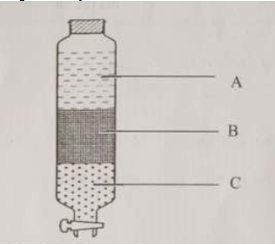
\includegraphics[width=0.5\textwidth]{./img/chem_I_matter_2.png}
	\end{center}
	Name the apparatus shown by the given figure. Giving a reason, identify liquids A and C. 
	
%%%%%%%%%%%%%%%%%%%%%%%%%%%%%%%%%%%%%%%%%%%%%%%%%%%%%%%%%%%%		
	\item Which method could be used to separate the products in the following equation? 
	\begin{center}
	Pb(NO$_3$)$_{2 (aq)}$ + 2KI$_{(aq)}$ $\rightarrow$ PbI$_{2 (S)}$ + 2KNO$_{3 (aq)}$ \\
	\textbf{colourless} \hspace*{2mm} \textbf{colourless} \hspace*{2mm} \textbf{yellow} \hspace*{2mm} \textbf{colourless}
	\end{center}
	\begin{enumerate}[topsep=0ex,itemsep=0ex,partopsep=1ex,parsep=1ex]
		\item[(A)] Chromatography
		\item[(B)] Crystallization
		\item[(C)] Distillation
		\item[(D)] Filtration
		\item[(E)] Condensation
	\end{enumerate}
	
	\item Briefly explain why the mixture with equal boiling point cannot be separated by simple fractional distillation
	
	\item Hygroscopic and deliquescent substances can be used as:
	\begin{enumerate}[topsep=0ex,itemsep=0ex,partopsep=1ex,parsep=1ex]
		\item[(A)] Oxidizing agents
		\item[(B)] Drying agents
		\item[(C)] Reducing agents
		\item[(D)] Weak electrolytes
		\item[(E)] Catalyst
	\end{enumerate}
	
	\item Water can be obtained from a solution of common salt by:
	\begin{enumerate}[topsep=0ex,itemsep=0ex,partopsep=1ex,parsep=1ex]
		\item[(A)] Evaporation
		\item[(B)] Simple distillation
		\item[(C)] Filtration
		\item[(D)] Condensation
		\item[(E)] Fractional distillation
	\end{enumerate}
	
	\item Suggest one best method for separating each of the following mixtures:
	\begin{enumerate}[topsep=0ex,itemsep=0ex,partopsep=1ex,parsep=1ex]
		\item[i)] Common salt and water
		\item[ii)] Iodine and sand
		\item[iii)] Pieces of iron and sand
	\end{enumerate}
\end{enumerate}

















